% Options for packages loaded elsewhere
\PassOptionsToPackage{unicode}{hyperref}
\PassOptionsToPackage{hyphens}{url}
%
\documentclass[
  12pt,
]{article}
\usepackage{lmodern}
\usepackage{amssymb,amsmath}
\usepackage{ifxetex,ifluatex}
\ifnum 0\ifxetex 1\fi\ifluatex 1\fi=0 % if pdftex
  \usepackage[T1]{fontenc}
  \usepackage[utf8]{inputenc}
  \usepackage{textcomp} % provide euro and other symbols
\else % if luatex or xetex
  \usepackage{unicode-math}
  \defaultfontfeatures{Scale=MatchLowercase}
  \defaultfontfeatures[\rmfamily]{Ligatures=TeX,Scale=1}
\fi
% Use upquote if available, for straight quotes in verbatim environments
\IfFileExists{upquote.sty}{\usepackage{upquote}}{}
\IfFileExists{microtype.sty}{% use microtype if available
  \usepackage[]{microtype}
  \UseMicrotypeSet[protrusion]{basicmath} % disable protrusion for tt fonts
}{}
\makeatletter
\@ifundefined{KOMAClassName}{% if non-KOMA class
  \IfFileExists{parskip.sty}{%
    \usepackage{parskip}
  }{% else
    \setlength{\parindent}{0pt}
    \setlength{\parskip}{6pt plus 2pt minus 1pt}}
}{% if KOMA class
  \KOMAoptions{parskip=half}}
\makeatother
\usepackage{xcolor}
\IfFileExists{xurl.sty}{\usepackage{xurl}}{} % add URL line breaks if available
\IfFileExists{bookmark.sty}{\usepackage{bookmark}}{\usepackage{hyperref}}
\hypersetup{
  pdftitle={Econometrics II TA Session \#13},
  pdfauthor={Hiroki Kato},
  hidelinks,
  pdfcreator={LaTeX via pandoc}}
\urlstyle{same} % disable monospaced font for URLs
\usepackage[margin=1in]{geometry}
\usepackage{color}
\usepackage{fancyvrb}
\newcommand{\VerbBar}{|}
\newcommand{\VERB}{\Verb[commandchars=\\\{\}]}
\DefineVerbatimEnvironment{Highlighting}{Verbatim}{commandchars=\\\{\}}
% Add ',fontsize=\small' for more characters per line
\usepackage{framed}
\definecolor{shadecolor}{RGB}{248,248,248}
\newenvironment{Shaded}{\begin{snugshade}}{\end{snugshade}}
\newcommand{\AlertTok}[1]{\textcolor[rgb]{0.94,0.16,0.16}{#1}}
\newcommand{\AnnotationTok}[1]{\textcolor[rgb]{0.56,0.35,0.01}{\textbf{\textit{#1}}}}
\newcommand{\AttributeTok}[1]{\textcolor[rgb]{0.77,0.63,0.00}{#1}}
\newcommand{\BaseNTok}[1]{\textcolor[rgb]{0.00,0.00,0.81}{#1}}
\newcommand{\BuiltInTok}[1]{#1}
\newcommand{\CharTok}[1]{\textcolor[rgb]{0.31,0.60,0.02}{#1}}
\newcommand{\CommentTok}[1]{\textcolor[rgb]{0.56,0.35,0.01}{\textit{#1}}}
\newcommand{\CommentVarTok}[1]{\textcolor[rgb]{0.56,0.35,0.01}{\textbf{\textit{#1}}}}
\newcommand{\ConstantTok}[1]{\textcolor[rgb]{0.00,0.00,0.00}{#1}}
\newcommand{\ControlFlowTok}[1]{\textcolor[rgb]{0.13,0.29,0.53}{\textbf{#1}}}
\newcommand{\DataTypeTok}[1]{\textcolor[rgb]{0.13,0.29,0.53}{#1}}
\newcommand{\DecValTok}[1]{\textcolor[rgb]{0.00,0.00,0.81}{#1}}
\newcommand{\DocumentationTok}[1]{\textcolor[rgb]{0.56,0.35,0.01}{\textbf{\textit{#1}}}}
\newcommand{\ErrorTok}[1]{\textcolor[rgb]{0.64,0.00,0.00}{\textbf{#1}}}
\newcommand{\ExtensionTok}[1]{#1}
\newcommand{\FloatTok}[1]{\textcolor[rgb]{0.00,0.00,0.81}{#1}}
\newcommand{\FunctionTok}[1]{\textcolor[rgb]{0.00,0.00,0.00}{#1}}
\newcommand{\ImportTok}[1]{#1}
\newcommand{\InformationTok}[1]{\textcolor[rgb]{0.56,0.35,0.01}{\textbf{\textit{#1}}}}
\newcommand{\KeywordTok}[1]{\textcolor[rgb]{0.13,0.29,0.53}{\textbf{#1}}}
\newcommand{\NormalTok}[1]{#1}
\newcommand{\OperatorTok}[1]{\textcolor[rgb]{0.81,0.36,0.00}{\textbf{#1}}}
\newcommand{\OtherTok}[1]{\textcolor[rgb]{0.56,0.35,0.01}{#1}}
\newcommand{\PreprocessorTok}[1]{\textcolor[rgb]{0.56,0.35,0.01}{\textit{#1}}}
\newcommand{\RegionMarkerTok}[1]{#1}
\newcommand{\SpecialCharTok}[1]{\textcolor[rgb]{0.00,0.00,0.00}{#1}}
\newcommand{\SpecialStringTok}[1]{\textcolor[rgb]{0.31,0.60,0.02}{#1}}
\newcommand{\StringTok}[1]{\textcolor[rgb]{0.31,0.60,0.02}{#1}}
\newcommand{\VariableTok}[1]{\textcolor[rgb]{0.00,0.00,0.00}{#1}}
\newcommand{\VerbatimStringTok}[1]{\textcolor[rgb]{0.31,0.60,0.02}{#1}}
\newcommand{\WarningTok}[1]{\textcolor[rgb]{0.56,0.35,0.01}{\textbf{\textit{#1}}}}
\usepackage{graphicx}
\makeatletter
\def\maxwidth{\ifdim\Gin@nat@width>\linewidth\linewidth\else\Gin@nat@width\fi}
\def\maxheight{\ifdim\Gin@nat@height>\textheight\textheight\else\Gin@nat@height\fi}
\makeatother
% Scale images if necessary, so that they will not overflow the page
% margins by default, and it is still possible to overwrite the defaults
% using explicit options in \includegraphics[width, height, ...]{}
\setkeys{Gin}{width=\maxwidth,height=\maxheight,keepaspectratio}
% Set default figure placement to htbp
\makeatletter
\def\fps@figure{htbp}
\makeatother
\setlength{\emergencystretch}{3em} % prevent overfull lines
\providecommand{\tightlist}{%
  \setlength{\itemsep}{0pt}\setlength{\parskip}{0pt}}
\setcounter{secnumdepth}{5}
\usepackage{zxjatype}
\setCJKmainfont[BoldFont = IPAゴシック]{IPA明朝}
\setCJKsansfont{IPAゴシック}
\setCJKmonofont{IPAゴシック}
\parindent = 1em
\newcommand{\argmax}{\mathop{\rm arg~max}\limits}
\newcommand{\argmin}{\mathop{\rm arg~min}\limits}
\DeclareMathOperator*{\plim}{plim}
\usepackage{xcolor}
\ifluatex
  \usepackage{selnolig}  % disable illegal ligatures
\fi

\title{Econometrics II TA Session \#13}
\author{Hiroki Kato}
\date{}

\begin{document}
\maketitle

\hypertarget{empirical-application-of-time-series-model-nikkei-225}{%
\section{Empirical Application of Time Series Model: Nikkei
225}\label{empirical-application-of-time-series-model-nikkei-225}}

\hypertarget{background-and-data}{%
\subsection{Background and Data}\label{background-and-data}}

The ``Nikkei225'' is a stock price index published by Nihon Keizai
Shimbun (hereafter, NIKKEI). NIKKEI calculates this price index based on
225 high liquid brands listed with first section of the Tokyo Stock
Exchange. We use daily data of the Nikkei 225 index taken from the yahoo
finance
(\url{https://stocks.finance.yahoo.co.jp/stocks/detail/?code=998407.O}).
The time length is from January 4th 2019 to January 22 2021. We have 498
observations. We read a csv data which recodes the Nikkei 225 dairy
index, using the \texttt{read.csv} function in \texttt{R}. Since
\texttt{R} recognize a time variable (e.g., \texttt{2021/01/22}) as a
character string, we need to define a time variable, using
\texttt{as.Date()} function. The data structure is as follows:

\begin{Shaded}
\begin{Highlighting}[]
\NormalTok{dt \textless{}{-}}\StringTok{ }\KeywordTok{read.csv}\NormalTok{(}\StringTok{"data/nikkei225.csv"}\NormalTok{, }\DataTypeTok{stringsAsFactor =} \OtherTok{FALSE}\NormalTok{)}
\NormalTok{dt}\OperatorTok{$}\NormalTok{date \textless{}{-}}\StringTok{ }\KeywordTok{as.Date}\NormalTok{(dt}\OperatorTok{$}\NormalTok{date, }\DataTypeTok{format =} \StringTok{"\%Y/\%m/\%d"}\NormalTok{)}
\KeywordTok{head}\NormalTok{(dt)}
\end{Highlighting}
\end{Shaded}

\begin{verbatim}
##         date open_price high_price low_price close_price
## 1 2021-01-22   28580.20   28698.18  28527.16    28631.45
## 2 2021-01-21   28710.41   28846.15  28677.61    28756.86
## 3 2021-01-20   28798.74   28801.19  28402.11    28523.26
## 4 2021-01-19   28405.49   28720.91  28373.34    28633.46
## 5 2021-01-18   28238.68   28349.97  28111.54    28242.21
## 6 2021-01-15   28777.47   28820.50  28477.03    28519.18
\end{verbatim}

There are five variables:

\begin{itemize}
\tightlist
\item
  \texttt{date}: date variable
\item
  \texttt{open\_price}: open price in day \(t\)
\item
  \texttt{high\_price}: high price in day \(t\)
\item
  \texttt{low\_price}: low price in day \(t\)
\item
  \texttt{close\_price}: closed price in day \(t\)
\end{itemize}

Mainly, we use the \texttt{date} and \texttt{close\_price}.

\begin{figure}[h]

{\centering 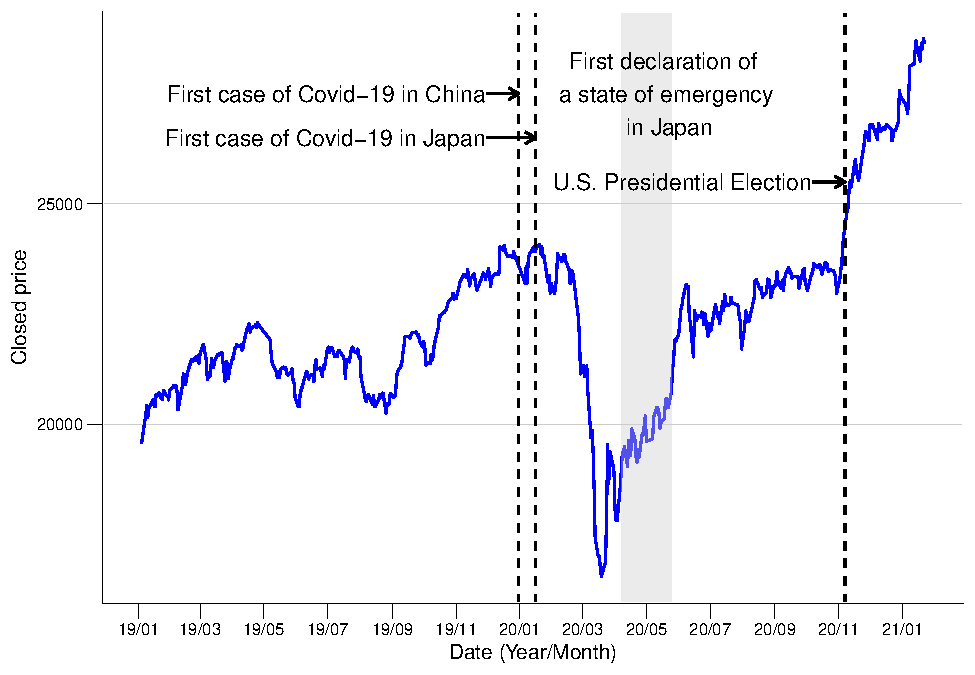
\includegraphics[width=0.9\linewidth]{C:/Users/katoo/Desktop/2020EconometricsTA/II/TAsession_13/handout_files/figure-latex/TimeSeriesPlot-1} 

}

\caption{Time Series Data of Nikkei 225}\label{fig:TimeSeriesPlot}
\end{figure}

Figure 1 shows the time series of closed price of the Nikkei225. We
summarize some features as follows:

\begin{itemize}
\tightlist
\item
  After the COVID-19 occured in Japan and China, the Nikkei225 has
  drastically decreased.
\item
  During the first declaration of a state of emergency in Japan, the
  Nikkei225's performance has been a V-shaped recovery.
\item
  The Nikkei225 has sharply increased immediaterly before and after the
  U.S. presidential election.
\end{itemize}

Some may wonder if the negative shock of COVID-19 reflects the
Nikkei225. To discuss it, we need to consider following two potential
concerns.

\begin{enumerate}
\def\labelenumi{\arabic{enumi}.}
\tightlist
\item
  unlisted companies (such as small restaurant business) may suffer
  heavily from the negative shock of COVID-19.
\item
  the Nikkei225 does not represent a variation of price index of 225
  brands. In principle, the Nikkei225 is a mathematical mean of stock
  price of 225 brands. In fact, the the stock prices of top five brands
  which contribute to the Nikkei225 have increased at 70\%. On the other
  hand, the stock price of other brands have decreased at 5\% from the
  begging of 2020 \footnote{See
    \url{https://news.yahoo.co.jp/articles/f63a4627b298857a62ac329b1ed41a88c2721bd4}.}.
\end{enumerate}

Anyway, we test the stationarity of this time series.

\hypertarget{autoregressive-of-order-1-ar1-model}{%
\subsection{Autoregressive of Order 1: AR(1)
model}\label{autoregressive-of-order-1-ar1-model}}

To check the stationarity of this time series, we consider the following
AR(1) model: \[ X_t = \beta X_{t-1} + \epsilon_t, \] where \(X_t\) is
the closed price of Nikkei225 in day \(t\). We assume \((\epsilon_t)\)
is a white noise process, \((\epsilon_t) \sim WN(0, \sigma^2)\). that
is, \(E(\epsilon_t) = 0\), \(E(\epsilon_t^2) = \sigma^2\), and
\(Cov(\epsilon_t, \epsilon_{t+h}) = 0\) for \(h \not= 0\).

To estimate the unkown parameters \(\theta = (\beta, \sigma^2)\), we use
the maximum likelihood method. We assume
\(\epsilon_t \sim N_{\mathbb{R}}N(0, \sigma^2)\) for inference purposes.
Then, the conditional log-likelihood is \[
  M_T(X_1, \ldots, X_T; \theta) 
  = \frac{1}{T} \sum_{t=2}^T \left\{ -\log(2\pi\sigma^2) - \frac{X_t - \beta X_{t-1}}{2\sigma^2} \right\}.
\] The MLE \(\hat{\theta}\) can be obtained by solving
\[ \hat{\theta} = \mathop{\rm arg~max}\limits_{\theta} M_T(X_1, \ldots, X_T; \theta). \]

\texttt{R} provides a built-in function to estimate AR(p) model, named
\texttt{ar()}. This function passes three augments, a time-series data,
estimation method, and autoregressive of order (p). To estimate AR(1)
model using the maximum likelihood method, we specify the number of
order, \texttt{order.max\ =\ 1}, and the method,
\texttt{method\ =\ "mle"}. The R snippet is as follows:

\begin{Shaded}
\begin{Highlighting}[]
\NormalTok{ar1 \textless{}{-}}\StringTok{ }\KeywordTok{ar}\NormalTok{(dt}\OperatorTok{$}\NormalTok{close\_price, }\DataTypeTok{method =} \StringTok{"mle"}\NormalTok{, }\DataTypeTok{order.max =} \DecValTok{1}\NormalTok{)}
\KeywordTok{sprintf}\NormalTok{(}\StringTok{"The estimated beta is \%1.4f (s.e. = \%1.4f)"}\NormalTok{, ar1}\OperatorTok{$}\NormalTok{ar, }\KeywordTok{sqrt}\NormalTok{(ar1}\OperatorTok{$}\NormalTok{asy.var.coef))}
\end{Highlighting}
\end{Shaded}

\begin{verbatim}
## [1] "The estimated beta is 0.9968 (s.e. = 0.0059)"
\end{verbatim}

\begin{Shaded}
\begin{Highlighting}[]
\KeywordTok{sprintf}\NormalTok{(}\StringTok{"The estimated squared sigma is \%1.2f"}\NormalTok{, ar1}\OperatorTok{$}\NormalTok{var.pred)}
\end{Highlighting}
\end{Shaded}

\begin{verbatim}
## [1] "The estimated squared sigma is 74014.82"
\end{verbatim}

\hypertarget{dickey-fuller-test}{%
\subsection{Dickey-Fuller test}\label{dickey-fuller-test}}

First, we derive the stationary condition in AR(1) model. The \(N\)-time
iterated substition of \(X_{t-1}\) yields
\[ X_t = \beta^N X_{t-N} + \sum_{k = 0}^N \beta^k \epsilon_{t-k}. \] If
\(|\beta| < 1\), then the first term of right hand side coverges to zero
as \(N \to \infty\). Thus, under \(|\beta| < 1\), the causal stationary
solution is \(X_t = \sum_{k=0}^{\infty} \beta^k \epsilon_{t-k}\).

Testing for stationarity is quivalent to test for \(\beta = 1\) in
AR(1). The null hypothesis is that the process is \textbf{not}
stationary. The alternative hypothesis is that the process is
stationary, that is, \(\beta < 1\). The Dickey-Fuller test provides this
\emph{one-sided} test.

To implement this test with \texttt{R}, we ues the package called
\texttt{tseries}. We use the function called \texttt{adf.test()} to
carry out the Dickey-Fuller test. We need to pass two augments in this
function. The first augment is time-series data. The second one, named
\texttt{k}, is the number of order (\(p\)). In this example, we pass
\texttt{k\ =\ 1}, that is, AR(1).

\begin{Shaded}
\begin{Highlighting}[]
\KeywordTok{library}\NormalTok{(tseries)}
\NormalTok{df1 \textless{}{-}}\StringTok{ }\KeywordTok{adf.test}\NormalTok{(dt}\OperatorTok{$}\NormalTok{close\_price, }\DataTypeTok{k =} \DecValTok{1}\NormalTok{)}
\KeywordTok{sprintf}\NormalTok{(}\StringTok{"The DF stats is \%1.4f (p{-}value = \%1.4f)"}\NormalTok{, df1}\OperatorTok{$}\NormalTok{statistic, df1}\OperatorTok{$}\NormalTok{p.value)}
\end{Highlighting}
\end{Shaded}

\begin{verbatim}
## [1] "The DF stats is -2.7638 (p-value = 0.2550)"
\end{verbatim}

As a result, we cannot reject the null hypothesis. Thus, the time series
of closed price of Nikkei225 is not stationary when we use data from
January 4th 2020 to January 22 2021.

\end{document}
